\documentclass{article}
\usepackage[margin=1in]{geometry}
\usepackage{amsmath,amsthm,amssymb}
\usepackage{bbm,enumerate,mathtools}
\usepackage{tikz,pgfplots}
\usepackage{chessboard}
\usepackage[hidelinks]{hyperref}
\usepackage{multicol} % Problem 35
\usepackage{xstring} % Difficulty command
\usetikzlibrary{shapes.geometric}

\newenvironment{question}{\begin{trivlist}\item[\textbf{Question.}]}{\end{trivlist}}
\newenvironment{note}{\begin{trivlist}\item[\textbf{Note.}]}{\end{trivlist}}
\newenvironment{references}{\begin{trivlist}\item[\textbf{References.}]}{\end{trivlist}}
\newenvironment{related}{\begin{trivlist}\item[\textbf{Related.}]\end{trivlist}\begin{enumerate}}{\end{enumerate}}

\newcommand\score[1]{
\pgfmathsetmacro\pgfxa{#1+1}
\tikzstyle{scorestars}=[
  star,
  star points=5,
  star point ratio=2.25,
  draw,
  inner sep=3pt,
  anchor=outer point 5
]
  \begin{tikzpicture}[baseline]
    \draw[opacity=0] (0,-0.5) rectangle (0,0.2); % Workaround for whitespace at the bottom.
    \foreach \i in {1,...,4} {
      \pgfmathparse{(\i<=#1?"yellow":"gray")}
      \edef\starcolor{\pgfmathresult}
      \draw (\i*4.5ex,0) node[name=star\i,scorestars,fill=\starcolor]  {};
    }
  \end{tikzpicture}
}

\newcommand{\difficulty}[1]{%
  \IfEqCase{#1}{%
      {1}{
        
\begin{tikzpicture}[scale=0.7, baseline=0.9mm]%
          \definecolor{slopegreen}{rgb}{0.0, 0.5, 0.0}%
          \fill[slopegreen] (0.5,0.5) circle (0.5);%
        \end{tikzpicture}%
      }%
      {2}{
        
\begin{tikzpicture}[scale=0.7, baseline=0.9mm]%
          \definecolor{slopeblue}{rgb}{0.0, 0.44, 1.00}
          \fill[slopeblue] (0,0) rectangle (1,1);%
        \end{tikzpicture}%
      }%
      {3}{
\begin{tikzpicture}[scale=0.7, baseline=0.9mm]\fill (0,0.5)--(0.5, 0)--(1,0.5)--(0.5,1)--cycle; \end{tikzpicture}}%
      {4}{
\begin{tikzpicture}[scale=0.7, baseline=0.9mm]\fill (0.25,0)--(0,0.5)--(0.25,1)--(0.5,0.5)--cycle; \fill (0.75,0)--(0.5,0.5)--(0.75,1)--(1,0.5)--cycle;\end{tikzpicture}}%
      % you can add more cases here as desired
  }[\PackageError{difficulty}{Undefined difficulty level: #1}{}]%
}%
\newcommand{\rating}[2]{\difficulty{#1}\\\score{#2}\\}


\begin{document}
\rating{4}{2}
Consider all rectangles composed of $n$ squares such that the greatest common
divisor of all the sidelengths is 1.

\begin{figure}[!h]
  \centering
  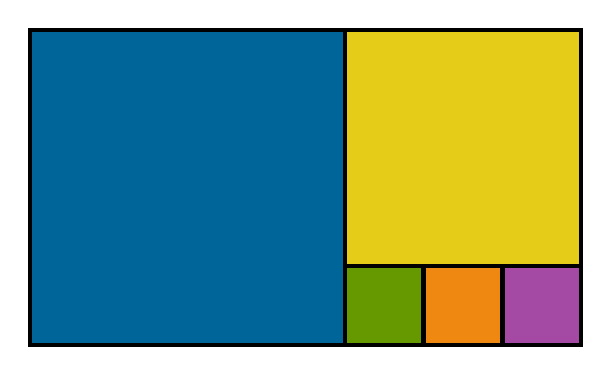
\begin{tikzpicture}
    \draw[ultra thick, fill={rgb:red,0;green,2;blue,3}] (0,0) rectangle (4,4);
    \draw[ultra thick, fill={rgb:red,1;yellow,8;blue,1}] (4,1) rectangle (7,4);
    \draw[ultra thick, fill={rgb:red,2;green,3;blue,0}] (4,0) rectangle (5,1);
    \draw[ultra thick, fill={rgb:red,6;yellow,8;blue,1}] (5,0) rectangle (6,1);
    \draw[ultra thick, fill={rgb:red,5;blue,5;white,4}] (6,0) rectangle (7,1);
  \end{tikzpicture}\hspace{1cm}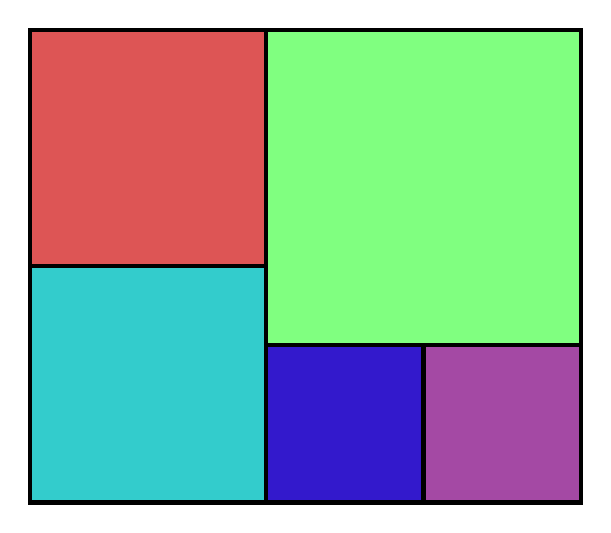
\begin{tikzpicture}
      \draw[ultra thick, fill={rgb:red,2;cyan,8}] (0,0) rectangle (3,3);
      \draw[ultra thick, fill={rgb:red,8;yellow,2;blue,2;white,3}] (0,3) rectangle (3,6);
      \draw[ultra thick, fill={rgb:red,0.5;yellow,0.5;blue,4}] (3,0) rectangle (5,2);
      \draw[ultra thick, fill={rgb:red,5;blue,5;white,4}] (5,0) rectangle (7,2);
      \draw[ultra thick, fill={rgb:green,5;white,5}] (3,2) rectangle (7,6);
    \end{tikzpicture}
  \caption{
    Two examples of rectangles made from $n=5$ squares.
    In the first $\gcd(1, 1, 1, 3, 4) = 1$ and in the second
    $\gcd(2,2,3,3,4) = 1$.
  }
\end{figure}

\begin{question}
  Given $n$ squares, how many such rectangles exist?
\end{question}
\begin{related}
  \item How many ways are there to make convex polygons out of $n$ equilateral triangles?
  \item How many ways are there to make cuboids out of $n$ cubes?
\end{related}
\end{document}
